\documentclass[twoside]{book}

% Packages required by doxygen
\usepackage{fixltx2e}
\usepackage{calc}
\usepackage{doxygen}
\usepackage[export]{adjustbox} % also loads graphicx
\usepackage{graphicx}
\usepackage[utf8]{inputenc}
\usepackage{makeidx}
\usepackage{multicol}
\usepackage{multirow}
\PassOptionsToPackage{warn}{textcomp}
\usepackage{textcomp}
\usepackage[nointegrals]{wasysym}
\usepackage[table]{xcolor}

% Font selection
\usepackage[T1]{fontenc}
\usepackage[scaled=.90]{helvet}
\usepackage{courier}
\usepackage{amssymb}
\usepackage{sectsty}
\renewcommand{\familydefault}{\sfdefault}
\allsectionsfont{%
  \fontseries{bc}\selectfont%
  \color{darkgray}%
}
\renewcommand{\DoxyLabelFont}{%
  \fontseries{bc}\selectfont%
  \color{darkgray}%
}
\newcommand{\+}{\discretionary{\mbox{\scriptsize$\hookleftarrow$}}{}{}}

% Page & text layout
\usepackage{geometry}
\geometry{%
  a4paper,%
  top=2.5cm,%
  bottom=2.5cm,%
  left=2.5cm,%
  right=2.5cm%
}
\tolerance=750
\hfuzz=15pt
\hbadness=750
\setlength{\emergencystretch}{15pt}
\setlength{\parindent}{0cm}
\setlength{\parskip}{3ex plus 2ex minus 2ex}
\makeatletter
\renewcommand{\paragraph}{%
  \@startsection{paragraph}{4}{0ex}{-1.0ex}{1.0ex}{%
    \normalfont\normalsize\bfseries\SS@parafont%
  }%
}
\renewcommand{\subparagraph}{%
  \@startsection{subparagraph}{5}{0ex}{-1.0ex}{1.0ex}{%
    \normalfont\normalsize\bfseries\SS@subparafont%
  }%
}
\makeatother

% Headers & footers
\usepackage{fancyhdr}
\pagestyle{fancyplain}
\fancyhead[LE]{\fancyplain{}{\bfseries\thepage}}
\fancyhead[CE]{\fancyplain{}{}}
\fancyhead[RE]{\fancyplain{}{\bfseries\leftmark}}
\fancyhead[LO]{\fancyplain{}{\bfseries\rightmark}}
\fancyhead[CO]{\fancyplain{}{}}
\fancyhead[RO]{\fancyplain{}{\bfseries\thepage}}
\fancyfoot[LE]{\fancyplain{}{}}
\fancyfoot[CE]{\fancyplain{}{}}
\fancyfoot[RE]{\fancyplain{}{\bfseries\scriptsize Generated by Doxygen }}
\fancyfoot[LO]{\fancyplain{}{\bfseries\scriptsize Generated by Doxygen }}
\fancyfoot[CO]{\fancyplain{}{}}
\fancyfoot[RO]{\fancyplain{}{}}
\renewcommand{\footrulewidth}{0.4pt}
\renewcommand{\chaptermark}[1]{%
  \markboth{#1}{}%
}
\renewcommand{\sectionmark}[1]{%
  \markright{\thesection\ #1}%
}

% Indices & bibliography
\usepackage{natbib}
\usepackage[titles]{tocloft}
\setcounter{tocdepth}{3}
\setcounter{secnumdepth}{5}
\makeindex

% Hyperlinks (required, but should be loaded last)
\usepackage{ifpdf}
\ifpdf
  \usepackage[pdftex,pagebackref=true]{hyperref}
\else
  \usepackage[ps2pdf,pagebackref=true]{hyperref}
\fi
\hypersetup{%
  colorlinks=true,%
  linkcolor=blue,%
  citecolor=blue,%
  unicode%
}

% Custom commands
\newcommand{\clearemptydoublepage}{%
  \newpage{\pagestyle{empty}\cleardoublepage}%
}

\usepackage{caption}
\captionsetup{labelsep=space,justification=centering,font={bf},singlelinecheck=off,skip=4pt,position=top}

%===== C O N T E N T S =====

\begin{document}

% Titlepage & ToC
\hypersetup{pageanchor=false,
             bookmarksnumbered=true,
             pdfencoding=unicode
            }
\pagenumbering{alph}
\begin{titlepage}
\vspace*{7cm}
\begin{center}%
{\Large My Project }\\
\vspace*{1cm}
{\large Generated by Doxygen 1.8.13}\\
\end{center}
\end{titlepage}
\clearemptydoublepage
\pagenumbering{roman}
\tableofcontents
\clearemptydoublepage
\pagenumbering{arabic}
\hypersetup{pageanchor=true}

%--- Begin generated contents ---
\chapter{Class Index}
\section{Class List}
Here are the classes, structs, unions and interfaces with brief descriptions\+:\begin{DoxyCompactList}
\item\contentsline{section}{\hyperlink{structbackground}{background} }{\pageref{structbackground}}{}
\item\contentsline{section}{\hyperlink{structpersonnage}{personnage} }{\pageref{structpersonnage}}{}
\item\contentsline{section}{\hyperlink{structscore__perso}{score\+\_\+perso} }{\pageref{structscore__perso}}{}
\item\contentsline{section}{\hyperlink{structthe}{the} \\*Struct for the background }{\pageref{structthe}}{}
\item\contentsline{section}{\hyperlink{structvie__perso}{vie\+\_\+perso} }{\pageref{structvie__perso}}{}
\end{DoxyCompactList}

\chapter{File Index}
\section{File List}
Here is a list of all documented files with brief descriptions\+:\begin{DoxyCompactList}
\item\contentsline{section}{\hyperlink{background_8c}{background.\+c} }{\pageref{background_8c}}{}
\item\contentsline{section}{{\bfseries background.\+h} }{\pageref{background_8h}}{}
\item\contentsline{section}{\hyperlink{main_8c}{main.\+c} }{\pageref{main_8c}}{}
\item\contentsline{section}{\hyperlink{perso_8c}{perso.\+c} }{\pageref{perso_8c}}{}
\item\contentsline{section}{{\bfseries perso.\+h} }{\pageref{perso_8h}}{}
\item\contentsline{section}{\hyperlink{stage1_8c}{stage1.\+c} }{\pageref{stage1_8c}}{}
\item\contentsline{section}{{\bfseries stage1.\+h} }{\pageref{stage1_8h}}{}
\item\contentsline{section}{\hyperlink{stat_8c}{stat.\+c} }{\pageref{stat_8c}}{}
\item\contentsline{section}{{\bfseries stat.\+h} }{\pageref{stat_8h}}{}
\end{DoxyCompactList}

\chapter{Class Documentation}
\hypertarget{structbackground}{}\section{background Struct Reference}
\label{structbackground}\index{background@{background}}
\subsection*{Public Attributes}
\begin{DoxyCompactItemize}
\item 
S\+D\+L\+\_\+\+Surface $\ast$ \hyperlink{structbackground_affdbb78ee8318f843c078291216b516a}{image\+\_\+back}
\item 
S\+D\+L\+\_\+\+Rect \hyperlink{structbackground_a32e36d3e27e3369de719761d14c374fe}{pos\+\_\+back}
\item 
\mbox{\Hypertarget{structbackground_a0d72cdea0f26aca19e8fb1b648a2c8b5}\label{structbackground_a0d72cdea0f26aca19e8fb1b648a2c8b5}} 
int {\bfseries gravity}
\end{DoxyCompactItemize}


\subsection{Member Data Documentation}
\mbox{\Hypertarget{structbackground_affdbb78ee8318f843c078291216b516a}\label{structbackground_affdbb78ee8318f843c078291216b516a}} 
\index{background@{background}!image\+\_\+back@{image\+\_\+back}}
\index{image\+\_\+back@{image\+\_\+back}!background@{background}}
\subsubsection{\texorpdfstring{image\+\_\+back}{image\_back}}
{\footnotesize\ttfamily S\+D\+L\+\_\+\+Surface$\ast$ background\+::image\+\_\+back}

Surface. \mbox{\Hypertarget{structbackground_a32e36d3e27e3369de719761d14c374fe}\label{structbackground_a32e36d3e27e3369de719761d14c374fe}} 
\index{background@{background}!pos\+\_\+back@{pos\+\_\+back}}
\index{pos\+\_\+back@{pos\+\_\+back}!background@{background}}
\subsubsection{\texorpdfstring{pos\+\_\+back}{pos\_back}}
{\footnotesize\ttfamily S\+D\+L\+\_\+\+Rect background\+::pos\+\_\+back}

Rectangle 

The documentation for this struct was generated from the following file\+:\begin{DoxyCompactItemize}
\item 
background.\+h\end{DoxyCompactItemize}

\hypertarget{structpersonnage}{}\section{personnage Struct Reference}
\label{structpersonnage}\index{personnage@{personnage}}
\subsection*{Public Attributes}
\begin{DoxyCompactItemize}
\item 
S\+D\+L\+\_\+\+Surface $\ast$ \hyperlink{structpersonnage_a791093b3684860157a3c156fe8bed344}{image\+\_\+perso}
\item 
S\+D\+L\+\_\+\+Rect \hyperlink{structpersonnage_ae463b597df9edc784f3d4e0ec1e4cb01}{pos\+\_\+perso}
\item 
S\+D\+L\+\_\+\+Rect \hyperlink{structpersonnage_af5e96572fb204c5b7b8f8c65df786c11}{pos\+\_\+perso\+\_\+relative}
\item 
\mbox{\Hypertarget{structpersonnage_a0ff04a353ae7233e1fc31f429e13fe36}\label{structpersonnage_a0ff04a353ae7233e1fc31f429e13fe36}} 
S\+D\+L\+\_\+\+Rect {\bfseries animation\+\_\+perso} \mbox{[}60\mbox{]}
\item 
\mbox{\Hypertarget{structpersonnage_a9be8353e105d1be0e4c8dd631d167b64}\label{structpersonnage_a9be8353e105d1be0e4c8dd631d167b64}} 
int {\bfseries comp\+\_\+tab\+\_\+animation\+\_\+perso}
\item 
\mbox{\Hypertarget{structpersonnage_a2664acffa6fccd8487b9e03b63fbd6da}\label{structpersonnage_a2664acffa6fccd8487b9e03b63fbd6da}} 
int {\bfseries direction}
\item 
\mbox{\Hypertarget{structpersonnage_a00f1b2301bdad28928de686202b50b07}\label{structpersonnage_a00f1b2301bdad28928de686202b50b07}} 
int {\bfseries stable}
\item 
\mbox{\Hypertarget{structpersonnage_a9cd9c9d66ebbb0faa4bdc9fd33230745}\label{structpersonnage_a9cd9c9d66ebbb0faa4bdc9fd33230745}} 
double {\bfseries vitesse\+\_\+perso}
\item 
\mbox{\Hypertarget{structpersonnage_afc0036b6619708ecb3239440c72383db}\label{structpersonnage_afc0036b6619708ecb3239440c72383db}} 
int {\bfseries vitesse\+\_\+max\+\_\+perso}
\item 
\mbox{\Hypertarget{structpersonnage_aa24491ca75878266706694b29b841691}\label{structpersonnage_aa24491ca75878266706694b29b841691}} 
int {\bfseries jump}
\item 
\mbox{\Hypertarget{structpersonnage_ad5c01f326fc913ef80791f84489c4c01}\label{structpersonnage_ad5c01f326fc913ef80791f84489c4c01}} 
int {\bfseries vie}
\item 
\mbox{\Hypertarget{structpersonnage_af36f152bd0d5da298cf6ebca6c566e79}\label{structpersonnage_af36f152bd0d5da298cf6ebca6c566e79}} 
int {\bfseries score}
\item 
\mbox{\Hypertarget{structpersonnage_a73b28615341c5003ce52f5ac6b759111}\label{structpersonnage_a73b28615341c5003ce52f5ac6b759111}} 
double {\bfseries acc}
\item 
\mbox{\Hypertarget{structpersonnage_ad149509f75e8aff1950b313aab0d7888}\label{structpersonnage_ad149509f75e8aff1950b313aab0d7888}} 
int {\bfseries acceleration}
\end{DoxyCompactItemize}


\subsection{Member Data Documentation}
\mbox{\Hypertarget{structpersonnage_a791093b3684860157a3c156fe8bed344}\label{structpersonnage_a791093b3684860157a3c156fe8bed344}} 
\index{personnage@{personnage}!image\+\_\+perso@{image\+\_\+perso}}
\index{image\+\_\+perso@{image\+\_\+perso}!personnage@{personnage}}
\subsubsection{\texorpdfstring{image\+\_\+perso}{image\_perso}}
{\footnotesize\ttfamily S\+D\+L\+\_\+\+Surface$\ast$ personnage\+::image\+\_\+perso}

Surface. \mbox{\Hypertarget{structpersonnage_ae463b597df9edc784f3d4e0ec1e4cb01}\label{structpersonnage_ae463b597df9edc784f3d4e0ec1e4cb01}} 
\index{personnage@{personnage}!pos\+\_\+perso@{pos\+\_\+perso}}
\index{pos\+\_\+perso@{pos\+\_\+perso}!personnage@{personnage}}
\subsubsection{\texorpdfstring{pos\+\_\+perso}{pos\_perso}}
{\footnotesize\ttfamily S\+D\+L\+\_\+\+Rect personnage\+::pos\+\_\+perso}

Rectangle \mbox{\Hypertarget{structpersonnage_af5e96572fb204c5b7b8f8c65df786c11}\label{structpersonnage_af5e96572fb204c5b7b8f8c65df786c11}} 
\index{personnage@{personnage}!pos\+\_\+perso\+\_\+relative@{pos\+\_\+perso\+\_\+relative}}
\index{pos\+\_\+perso\+\_\+relative@{pos\+\_\+perso\+\_\+relative}!personnage@{personnage}}
\subsubsection{\texorpdfstring{pos\+\_\+perso\+\_\+relative}{pos\_perso\_relative}}
{\footnotesize\ttfamily S\+D\+L\+\_\+\+Rect personnage\+::pos\+\_\+perso\+\_\+relative}

Rectangle 

The documentation for this struct was generated from the following file\+:\begin{DoxyCompactItemize}
\item 
perso.\+h\end{DoxyCompactItemize}

\hypertarget{structscore__perso}{}\section{score\+\_\+perso Struct Reference}
\label{structscore__perso}\index{score\+\_\+perso@{score\+\_\+perso}}
\subsection*{Public Attributes}
\begin{DoxyCompactItemize}
\item 
\mbox{\Hypertarget{structscore__perso_a7bdcd5e9dfad29e5043e082b1639819c}\label{structscore__perso_a7bdcd5e9dfad29e5043e082b1639819c}} 
T\+T\+F\+\_\+\+Font $\ast$ {\bfseries police\+\_\+score}
\item 
\mbox{\Hypertarget{structscore__perso_a746add510ddf10a1ac7e985e2ae73036}\label{structscore__perso_a746add510ddf10a1ac7e985e2ae73036}} 
S\+D\+L\+\_\+\+Surface $\ast$ {\bfseries texte\+\_\+score}
\item 
\mbox{\Hypertarget{structscore__perso_a1395bca9a5dbb6b447d88d54003eac53}\label{structscore__perso_a1395bca9a5dbb6b447d88d54003eac53}} 
S\+D\+L\+\_\+\+Rect {\bfseries pos\+\_\+texte\+\_\+score}
\end{DoxyCompactItemize}


The documentation for this struct was generated from the following file\+:\begin{DoxyCompactItemize}
\item 
stat.\+h\end{DoxyCompactItemize}

\hypertarget{structthe}{}\section{the Struct Reference}
\label{structthe}\index{the@{the}}


struct for the background  




\subsection{Detailed Description}
struct for the background 

struct for the \hyperlink{structscore__perso}{score\+\_\+perso}

struct for the \hyperlink{structvie__perso}{vie\+\_\+perso}

struct for the personnage 

The documentation for this struct was generated from the following file\+:\begin{DoxyCompactItemize}
\item 
background.\+h\end{DoxyCompactItemize}

\hypertarget{structvie__perso}{}\section{vie\+\_\+perso Struct Reference}
\label{structvie__perso}\index{vie\+\_\+perso@{vie\+\_\+perso}}
\subsection*{Public Attributes}
\begin{DoxyCompactItemize}
\item 
\mbox{\Hypertarget{structvie__perso_afd57a88c68a51436785e97929e6bb74d}\label{structvie__perso_afd57a88c68a51436785e97929e6bb74d}} 
T\+T\+F\+\_\+\+Font $\ast$ {\bfseries police\+\_\+vie}
\item 
\mbox{\Hypertarget{structvie__perso_a376ee3a635e48edafe9a5e6264356056}\label{structvie__perso_a376ee3a635e48edafe9a5e6264356056}} 
S\+D\+L\+\_\+\+Surface $\ast$ {\bfseries texte\+\_\+vie}
\item 
\mbox{\Hypertarget{structvie__perso_ac2eb84bf9052be13ad455458c9de4f38}\label{structvie__perso_ac2eb84bf9052be13ad455458c9de4f38}} 
S\+D\+L\+\_\+\+Rect {\bfseries pos\+\_\+texte\+\_\+vie}
\end{DoxyCompactItemize}


The documentation for this struct was generated from the following file\+:\begin{DoxyCompactItemize}
\item 
stat.\+h\end{DoxyCompactItemize}

\chapter{File Documentation}
\hypertarget{background_8c}{}\section{background.\+c File Reference}
\label{background_8c}\index{background.\+c@{background.\+c}}
{\ttfamily \#include \char`\"{}background.\+h\char`\"{}}\newline
Include dependency graph for background.\+c\+:
\nopagebreak
\begin{figure}[H]
\begin{center}
\leavevmode
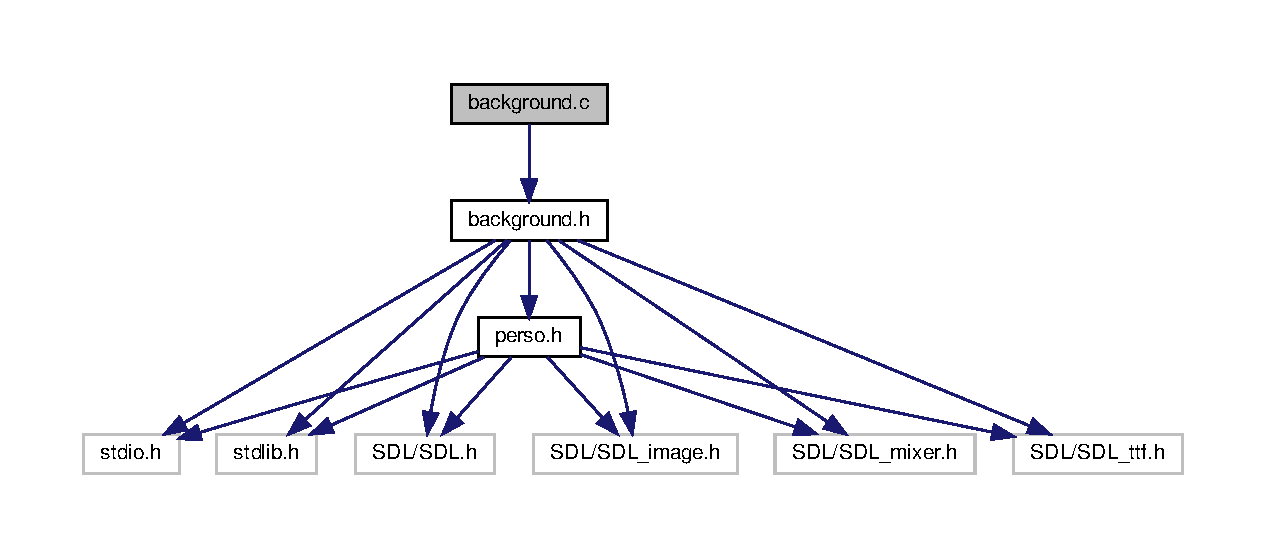
\includegraphics[width=350pt]{background_8c__incl}
\end{center}
\end{figure}
\subsection*{Functions}
\begin{DoxyCompactItemize}
\item 
void \hyperlink{background_8c_aa4d19046469a112c54c82d2d1883b260}{initialiser\+\_\+back} (\hyperlink{structbackground}{background} $\ast$bg)
\begin{DoxyCompactList}\small\item\em To initialize the backdround bg . \end{DoxyCompactList}\item 
void \hyperlink{background_8c_a3ea78313873b579b47ac72247aabf720}{afficher\+\_\+back} (\hyperlink{structbackground}{background} $\ast$bg, S\+D\+L\+\_\+\+Surface $\ast$screen)
\begin{DoxyCompactList}\small\item\em To show the backdround bg . \end{DoxyCompactList}\item 
void \hyperlink{background_8c_a45a617730ae1f0ff2c6d7c89baf5e7af}{gravity} (\hyperlink{structpersonnage}{personnage} $\ast$p, \hyperlink{structbackground}{background} bg)
\begin{DoxyCompactList}\small\item\em for the gravity . \end{DoxyCompactList}\end{DoxyCompactItemize}


\subsection{Function Documentation}
\mbox{\Hypertarget{background_8c_a3ea78313873b579b47ac72247aabf720}\label{background_8c_a3ea78313873b579b47ac72247aabf720}} 
\index{background.\+c@{background.\+c}!afficher\+\_\+back@{afficher\+\_\+back}}
\index{afficher\+\_\+back@{afficher\+\_\+back}!background.\+c@{background.\+c}}
\subsubsection{\texorpdfstring{afficher\+\_\+back()}{afficher\_back()}}
{\footnotesize\ttfamily void afficher\+\_\+back (\begin{DoxyParamCaption}\item[{\hyperlink{structbackground}{background} $\ast$}]{bg,  }\item[{S\+D\+L\+\_\+\+Surface $\ast$}]{screen }\end{DoxyParamCaption})}



To show the backdround bg . 


\begin{DoxyParams}{Parameters}
{\em screen} & the screen \\
\hline
{\em bg} & backdround bg \\
\hline
\end{DoxyParams}
\begin{DoxyReturn}{Returns}
Nothing 
\end{DoxyReturn}
\mbox{\Hypertarget{background_8c_a45a617730ae1f0ff2c6d7c89baf5e7af}\label{background_8c_a45a617730ae1f0ff2c6d7c89baf5e7af}} 
\index{background.\+c@{background.\+c}!gravity@{gravity}}
\index{gravity@{gravity}!background.\+c@{background.\+c}}
\subsubsection{\texorpdfstring{gravity()}{gravity()}}
{\footnotesize\ttfamily void gravity (\begin{DoxyParamCaption}\item[{\hyperlink{structpersonnage}{personnage} $\ast$}]{p,  }\item[{\hyperlink{structbackground}{background}}]{bg }\end{DoxyParamCaption})}



for the gravity . 


\begin{DoxyParams}{Parameters}
{\em bg} & the background \\
\hline
{\em p} & the personnage \\
\hline
\end{DoxyParams}
\begin{DoxyReturn}{Returns}
Nothing 
\end{DoxyReturn}
\mbox{\Hypertarget{background_8c_aa4d19046469a112c54c82d2d1883b260}\label{background_8c_aa4d19046469a112c54c82d2d1883b260}} 
\index{background.\+c@{background.\+c}!initialiser\+\_\+back@{initialiser\+\_\+back}}
\index{initialiser\+\_\+back@{initialiser\+\_\+back}!background.\+c@{background.\+c}}
\subsubsection{\texorpdfstring{initialiser\+\_\+back()}{initialiser\_back()}}
{\footnotesize\ttfamily void initialiser\+\_\+back (\begin{DoxyParamCaption}\item[{\hyperlink{structbackground}{background} $\ast$}]{bg }\end{DoxyParamCaption})}



To initialize the backdround bg . 


\begin{DoxyParams}{Parameters}
{\em bg} & the background \\
\hline
\end{DoxyParams}
\begin{DoxyReturn}{Returns}
Nothing 
\end{DoxyReturn}

\hypertarget{main_8c}{}\section{main.\+c File Reference}
\label{main_8c}\index{main.\+c@{main.\+c}}
{\ttfamily \#include $<$stdio.\+h$>$}\newline
{\ttfamily \#include $<$stdlib.\+h$>$}\newline
{\ttfamily \#include $<$S\+D\+L/\+S\+D\+L.\+h$>$}\newline
{\ttfamily \#include $<$S\+D\+L/\+S\+D\+L\+\_\+image.\+h$>$}\newline
{\ttfamily \#include $<$S\+D\+L/\+S\+D\+L\+\_\+mixer.\+h$>$}\newline
{\ttfamily \#include $<$S\+D\+L/\+S\+D\+L\+\_\+ttf.\+h$>$}\newline
{\ttfamily \#include \char`\"{}stage1.\+h\char`\"{}}\newline
Include dependency graph for main.\+c\+:
\nopagebreak
\begin{figure}[H]
\begin{center}
\leavevmode
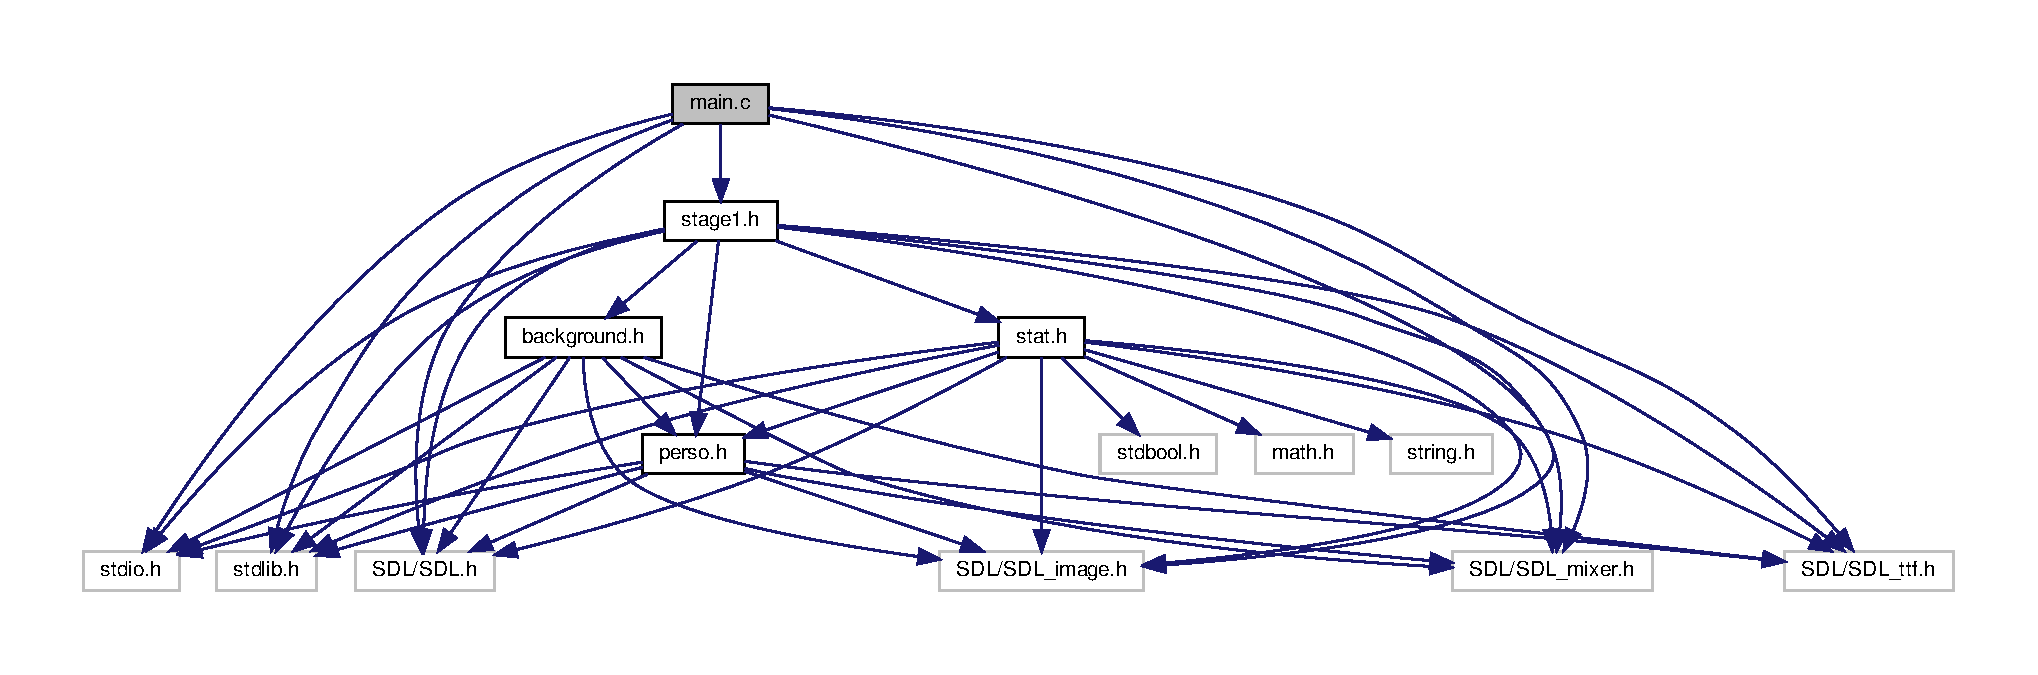
\includegraphics[width=350pt]{main_8c__incl}
\end{center}
\end{figure}
\subsection*{Functions}
\begin{DoxyCompactItemize}
\item 
\mbox{\Hypertarget{main_8c_ae66f6b31b5ad750f1fe042a706a4e3d4}\label{main_8c_ae66f6b31b5ad750f1fe042a706a4e3d4}} 
int {\bfseries main} ()
\end{DoxyCompactItemize}

\hypertarget{perso_8c}{}\section{perso.\+c File Reference}
\label{perso_8c}\index{perso.\+c@{perso.\+c}}
{\ttfamily \#include \char`\"{}perso.\+h\char`\"{}}\newline
Include dependency graph for perso.\+c\+:
\nopagebreak
\begin{figure}[H]
\begin{center}
\leavevmode
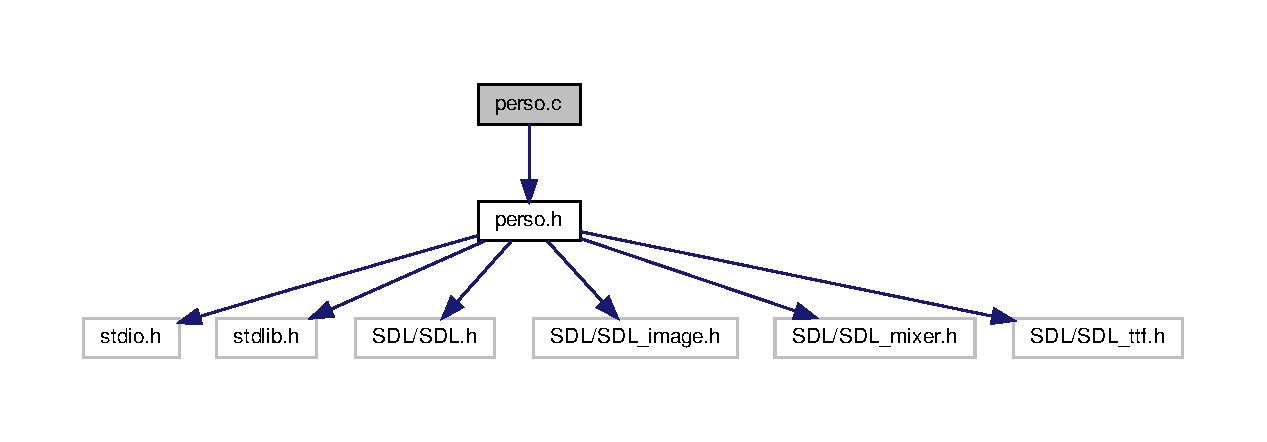
\includegraphics[width=350pt]{perso_8c__incl}
\end{center}
\end{figure}
\subsection*{Functions}
\begin{DoxyCompactItemize}
\item 
\mbox{\Hypertarget{perso_8c_a85e6aaf9b4118a4114712f5bc22ad11f}\label{perso_8c_a85e6aaf9b4118a4114712f5bc22ad11f}} 
void {\bfseries initialiser\+\_\+animation\+\_\+perso} (S\+D\+L\+\_\+\+Rect $\ast$clip)
\item 
void \hyperlink{perso_8c_ab76e735545868fc99b5b91849eea7d7a}{initialiser\+\_\+perso} (\hyperlink{structpersonnage}{personnage} $\ast$p)
\begin{DoxyCompactList}\small\item\em To initialize the personnage p . \end{DoxyCompactList}\item 
void \hyperlink{perso_8c_a43181619fa488bdbf458203b3a0a51c5}{afficher\+\_\+perso} (\hyperlink{structpersonnage}{personnage} $\ast$p, S\+D\+L\+\_\+\+Surface $\ast$screen)
\begin{DoxyCompactList}\small\item\em To show the personnage p . \end{DoxyCompactList}\item 
void \hyperlink{perso_8c_ad47ed90717588a44782d7fc447b9da38}{avancer\+\_\+perso} (\hyperlink{structpersonnage}{personnage} $\ast$p, Uint32 dt)
\begin{DoxyCompactList}\small\item\em for the movement of the personnage p (right) . \end{DoxyCompactList}\item 
void \hyperlink{perso_8c_af2d468b1b3c2ac314c537523935f30a3}{reculer\+\_\+perso} (\hyperlink{structpersonnage}{personnage} $\ast$p, Uint32 dt)
\begin{DoxyCompactList}\small\item\em for the movement of the personnage p (left) . \end{DoxyCompactList}\item 
void \hyperlink{perso_8c_a0bd10122e93a415b8fb3b7b1b99d0343}{animation\+\_\+perso\+\_\+stable} (\hyperlink{structpersonnage}{personnage} $\ast$p)
\begin{DoxyCompactList}\small\item\em for the annimation of the personnage when he is (stable ) . \end{DoxyCompactList}\item 
void \hyperlink{perso_8c_acf78a9d4298ec00e8c547fc2047dc165}{animation\+\_\+perso\+\_\+mvt\+\_\+droite} (\hyperlink{structpersonnage}{personnage} $\ast$p)
\begin{DoxyCompactList}\small\item\em for annimation of the personnage when he moove to the right . . \end{DoxyCompactList}\item 
void \hyperlink{perso_8c_aca82958e9c2d40dd84411f1dbead06fd}{animation\+\_\+perso\+\_\+mvt\+\_\+gauche} (\hyperlink{structpersonnage}{personnage} $\ast$p)
\begin{DoxyCompactList}\small\item\em for annimation of the personnage when he moove to the right . . \end{DoxyCompactList}\item 
void \hyperlink{perso_8c_a5dbb91d858957a453f8ff0fab86b1b4f}{acceleration} (\hyperlink{structpersonnage}{personnage} $\ast$p, Uint32 dt)
\begin{DoxyCompactList}\small\item\em for the acceleration of the personnage . . \end{DoxyCompactList}\item 
void \hyperlink{perso_8c_a43aa4382fb26d1e6f57c9a8ffff1abd9}{jump\+\_\+perso} (\hyperlink{structpersonnage}{personnage} $\ast$p)
\begin{DoxyCompactList}\small\item\em for the jump of the personnage . . \end{DoxyCompactList}\end{DoxyCompactItemize}
\subsection*{Variables}
\begin{DoxyCompactItemize}
\item 
\mbox{\Hypertarget{perso_8c_ab428534f5943def0966f97bbd6121b8d}\label{perso_8c_ab428534f5943def0966f97bbd6121b8d}} 
int {\bfseries nb\+\_\+image\+\_\+par\+\_\+ligne\+\_\+spritesheet} =11
\item 
\mbox{\Hypertarget{perso_8c_ab5ad6832fa73f7509f57d1f8fb835659}\label{perso_8c_ab5ad6832fa73f7509f57d1f8fb835659}} 
int {\bfseries nb\+\_\+ligne\+\_\+spritesheet} =4
\end{DoxyCompactItemize}


\subsection{Function Documentation}
\mbox{\Hypertarget{perso_8c_a5dbb91d858957a453f8ff0fab86b1b4f}\label{perso_8c_a5dbb91d858957a453f8ff0fab86b1b4f}} 
\index{perso.\+c@{perso.\+c}!acceleration@{acceleration}}
\index{acceleration@{acceleration}!perso.\+c@{perso.\+c}}
\subsubsection{\texorpdfstring{acceleration()}{acceleration()}}
{\footnotesize\ttfamily void acceleration (\begin{DoxyParamCaption}\item[{\hyperlink{structpersonnage}{personnage} $\ast$}]{p,  }\item[{Uint32}]{dt }\end{DoxyParamCaption})}



for the acceleration of the personnage . . 


\begin{DoxyParams}{Parameters}
{\em p} & the personnage \\
\hline
{\em dt} & Unit32 \\
\hline
\end{DoxyParams}
\begin{DoxyReturn}{Returns}
Nothing 
\end{DoxyReturn}
\mbox{\Hypertarget{perso_8c_a43181619fa488bdbf458203b3a0a51c5}\label{perso_8c_a43181619fa488bdbf458203b3a0a51c5}} 
\index{perso.\+c@{perso.\+c}!afficher\+\_\+perso@{afficher\+\_\+perso}}
\index{afficher\+\_\+perso@{afficher\+\_\+perso}!perso.\+c@{perso.\+c}}
\subsubsection{\texorpdfstring{afficher\+\_\+perso()}{afficher\_perso()}}
{\footnotesize\ttfamily void afficher\+\_\+perso (\begin{DoxyParamCaption}\item[{\hyperlink{structpersonnage}{personnage} $\ast$}]{p,  }\item[{S\+D\+L\+\_\+\+Surface $\ast$}]{screen }\end{DoxyParamCaption})}



To show the personnage p . 


\begin{DoxyParams}{Parameters}
{\em screen} & the screen \\
\hline
{\em p} & the personnage \\
\hline
\end{DoxyParams}
\begin{DoxyReturn}{Returns}
Nothing 
\end{DoxyReturn}
\mbox{\Hypertarget{perso_8c_acf78a9d4298ec00e8c547fc2047dc165}\label{perso_8c_acf78a9d4298ec00e8c547fc2047dc165}} 
\index{perso.\+c@{perso.\+c}!animation\+\_\+perso\+\_\+mvt\+\_\+droite@{animation\+\_\+perso\+\_\+mvt\+\_\+droite}}
\index{animation\+\_\+perso\+\_\+mvt\+\_\+droite@{animation\+\_\+perso\+\_\+mvt\+\_\+droite}!perso.\+c@{perso.\+c}}
\subsubsection{\texorpdfstring{animation\+\_\+perso\+\_\+mvt\+\_\+droite()}{animation\_perso\_mvt\_droite()}}
{\footnotesize\ttfamily void animation\+\_\+perso\+\_\+mvt\+\_\+droite (\begin{DoxyParamCaption}\item[{\hyperlink{structpersonnage}{personnage} $\ast$}]{p }\end{DoxyParamCaption})}



for annimation of the personnage when he moove to the right . . 


\begin{DoxyParams}{Parameters}
{\em p} & the personnage \\
\hline
\end{DoxyParams}
\begin{DoxyReturn}{Returns}
Nothing 
\end{DoxyReturn}
\mbox{\Hypertarget{perso_8c_aca82958e9c2d40dd84411f1dbead06fd}\label{perso_8c_aca82958e9c2d40dd84411f1dbead06fd}} 
\index{perso.\+c@{perso.\+c}!animation\+\_\+perso\+\_\+mvt\+\_\+gauche@{animation\+\_\+perso\+\_\+mvt\+\_\+gauche}}
\index{animation\+\_\+perso\+\_\+mvt\+\_\+gauche@{animation\+\_\+perso\+\_\+mvt\+\_\+gauche}!perso.\+c@{perso.\+c}}
\subsubsection{\texorpdfstring{animation\+\_\+perso\+\_\+mvt\+\_\+gauche()}{animation\_perso\_mvt\_gauche()}}
{\footnotesize\ttfamily void animation\+\_\+perso\+\_\+mvt\+\_\+gauche (\begin{DoxyParamCaption}\item[{\hyperlink{structpersonnage}{personnage} $\ast$}]{p }\end{DoxyParamCaption})}



for annimation of the personnage when he moove to the right . . 


\begin{DoxyParams}{Parameters}
{\em p} & the personnage \\
\hline
\end{DoxyParams}
\begin{DoxyReturn}{Returns}
Nothing 
\end{DoxyReturn}
\mbox{\Hypertarget{perso_8c_a0bd10122e93a415b8fb3b7b1b99d0343}\label{perso_8c_a0bd10122e93a415b8fb3b7b1b99d0343}} 
\index{perso.\+c@{perso.\+c}!animation\+\_\+perso\+\_\+stable@{animation\+\_\+perso\+\_\+stable}}
\index{animation\+\_\+perso\+\_\+stable@{animation\+\_\+perso\+\_\+stable}!perso.\+c@{perso.\+c}}
\subsubsection{\texorpdfstring{animation\+\_\+perso\+\_\+stable()}{animation\_perso\_stable()}}
{\footnotesize\ttfamily void animation\+\_\+perso\+\_\+stable (\begin{DoxyParamCaption}\item[{\hyperlink{structpersonnage}{personnage} $\ast$}]{p }\end{DoxyParamCaption})}



for the annimation of the personnage when he is (stable ) . 


\begin{DoxyParams}{Parameters}
{\em p} & the personnage \\
\hline
\end{DoxyParams}
\begin{DoxyReturn}{Returns}
Nothing 
\end{DoxyReturn}
\mbox{\Hypertarget{perso_8c_ad47ed90717588a44782d7fc447b9da38}\label{perso_8c_ad47ed90717588a44782d7fc447b9da38}} 
\index{perso.\+c@{perso.\+c}!avancer\+\_\+perso@{avancer\+\_\+perso}}
\index{avancer\+\_\+perso@{avancer\+\_\+perso}!perso.\+c@{perso.\+c}}
\subsubsection{\texorpdfstring{avancer\+\_\+perso()}{avancer\_perso()}}
{\footnotesize\ttfamily void avancer\+\_\+perso (\begin{DoxyParamCaption}\item[{\hyperlink{structpersonnage}{personnage} $\ast$}]{p,  }\item[{Uint32}]{dt }\end{DoxyParamCaption})}



for the movement of the personnage p (right) . 


\begin{DoxyParams}{Parameters}
{\em dt} & Unit32 \\
\hline
{\em p} & the personnage \\
\hline
\end{DoxyParams}
\begin{DoxyReturn}{Returns}
Nothing 
\end{DoxyReturn}
\mbox{\Hypertarget{perso_8c_ab76e735545868fc99b5b91849eea7d7a}\label{perso_8c_ab76e735545868fc99b5b91849eea7d7a}} 
\index{perso.\+c@{perso.\+c}!initialiser\+\_\+perso@{initialiser\+\_\+perso}}
\index{initialiser\+\_\+perso@{initialiser\+\_\+perso}!perso.\+c@{perso.\+c}}
\subsubsection{\texorpdfstring{initialiser\+\_\+perso()}{initialiser\_perso()}}
{\footnotesize\ttfamily void initialiser\+\_\+perso (\begin{DoxyParamCaption}\item[{\hyperlink{structpersonnage}{personnage} $\ast$}]{p }\end{DoxyParamCaption})}



To initialize the personnage p . 


\begin{DoxyParams}{Parameters}
{\em p} & the personnage \\
\hline
\end{DoxyParams}
\begin{DoxyReturn}{Returns}
Nothing 
\end{DoxyReturn}
\mbox{\Hypertarget{perso_8c_a43aa4382fb26d1e6f57c9a8ffff1abd9}\label{perso_8c_a43aa4382fb26d1e6f57c9a8ffff1abd9}} 
\index{perso.\+c@{perso.\+c}!jump\+\_\+perso@{jump\+\_\+perso}}
\index{jump\+\_\+perso@{jump\+\_\+perso}!perso.\+c@{perso.\+c}}
\subsubsection{\texorpdfstring{jump\+\_\+perso()}{jump\_perso()}}
{\footnotesize\ttfamily void jump\+\_\+perso (\begin{DoxyParamCaption}\item[{\hyperlink{structpersonnage}{personnage} $\ast$}]{p }\end{DoxyParamCaption})}



for the jump of the personnage . . 


\begin{DoxyParams}{Parameters}
{\em p} & the personnage \\
\hline
\end{DoxyParams}
\begin{DoxyReturn}{Returns}
Nothing 
\end{DoxyReturn}
\mbox{\Hypertarget{perso_8c_af2d468b1b3c2ac314c537523935f30a3}\label{perso_8c_af2d468b1b3c2ac314c537523935f30a3}} 
\index{perso.\+c@{perso.\+c}!reculer\+\_\+perso@{reculer\+\_\+perso}}
\index{reculer\+\_\+perso@{reculer\+\_\+perso}!perso.\+c@{perso.\+c}}
\subsubsection{\texorpdfstring{reculer\+\_\+perso()}{reculer\_perso()}}
{\footnotesize\ttfamily void reculer\+\_\+perso (\begin{DoxyParamCaption}\item[{\hyperlink{structpersonnage}{personnage} $\ast$}]{p,  }\item[{Uint32}]{dt }\end{DoxyParamCaption})}



for the movement of the personnage p (left) . 


\begin{DoxyParams}{Parameters}
{\em dt} & Unit32 \\
\hline
{\em p} & the personnage \\
\hline
\end{DoxyParams}
\begin{DoxyReturn}{Returns}
Nothing 
\end{DoxyReturn}

\hypertarget{stage1_8c}{}\section{stage1.\+c File Reference}
\label{stage1_8c}\index{stage1.\+c@{stage1.\+c}}
{\ttfamily \#include \char`\"{}stage1.\+h\char`\"{}}\newline
Include dependency graph for stage1.\+c\+:
\nopagebreak
\begin{figure}[H]
\begin{center}
\leavevmode
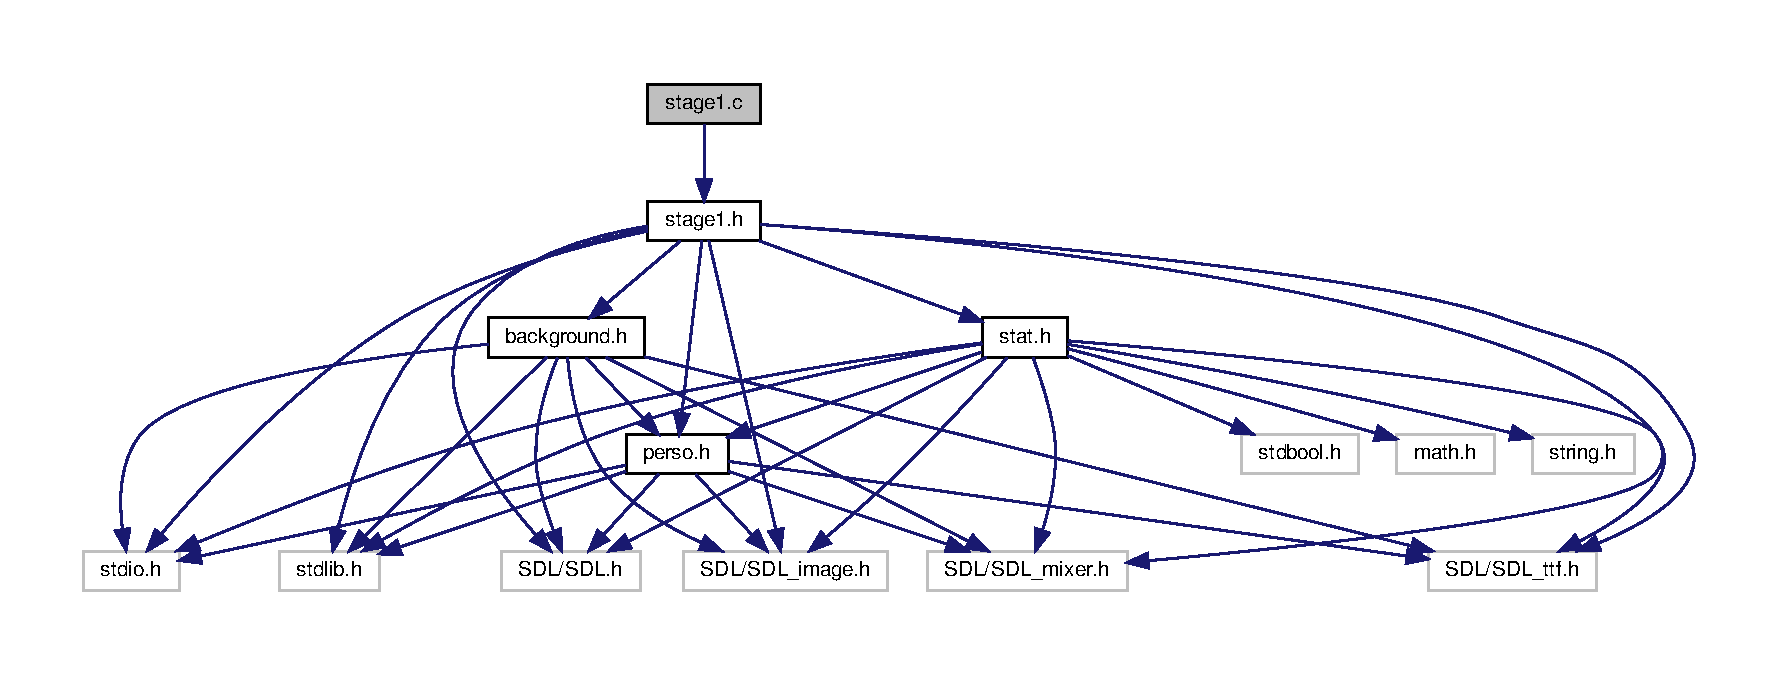
\includegraphics[width=350pt]{stage1_8c__incl}
\end{center}
\end{figure}
\subsection*{Functions}
\begin{DoxyCompactItemize}
\item 
\mbox{\Hypertarget{stage1_8c_ab932a377f3b88227b9c475d545124267}\label{stage1_8c_ab932a377f3b88227b9c475d545124267}} 
int {\bfseries stage\+\_\+1} (S\+D\+L\+\_\+\+Surface $\ast$screen)
\end{DoxyCompactItemize}

\hypertarget{stat_8c}{}\section{stat.\+c File Reference}
\label{stat_8c}\index{stat.\+c@{stat.\+c}}
{\ttfamily \#include \char`\"{}stat.\+h\char`\"{}}\newline
Include dependency graph for stat.\+c\+:
\nopagebreak
\begin{figure}[H]
\begin{center}
\leavevmode
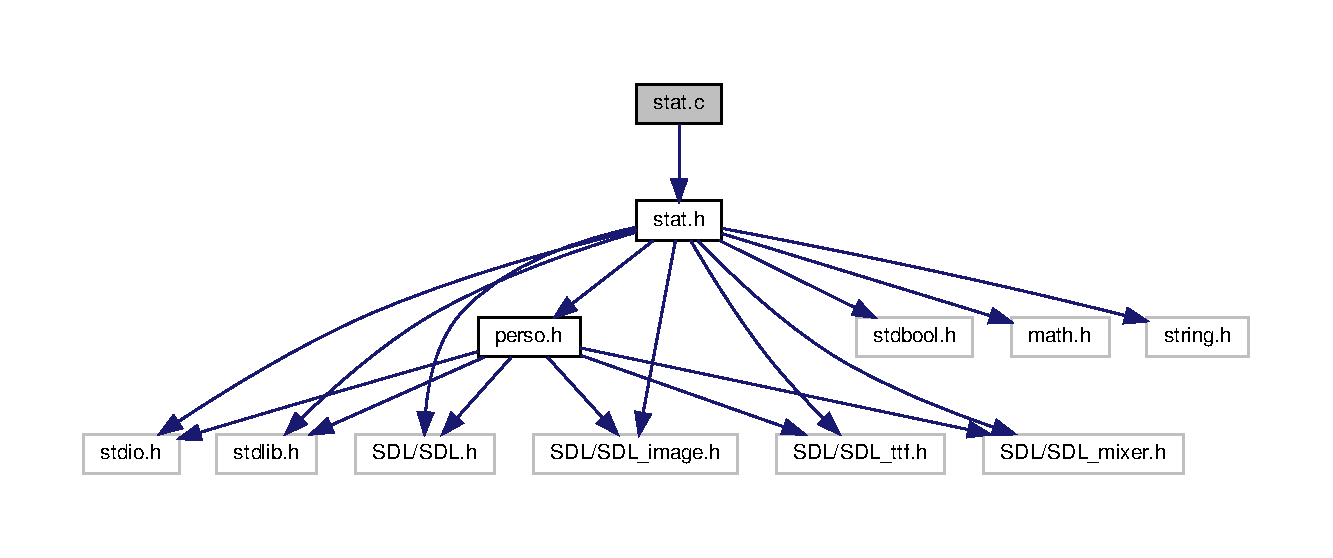
\includegraphics[width=350pt]{stat_8c__incl}
\end{center}
\end{figure}
\subsection*{Functions}
\begin{DoxyCompactItemize}
\item 
void \hyperlink{stat_8c_a28472946db8351efce564ed558a5c0e8}{init\+\_\+vie} (\hyperlink{structvie__perso}{vie\+\_\+perso} $\ast$v)
\begin{DoxyCompactList}\small\item\em To initialize the \hyperlink{structvie__perso}{vie\+\_\+perso} v . \end{DoxyCompactList}\item 
void \hyperlink{stat_8c_ac3769f909fa81048d93b903145b47759}{init\+\_\+score} (\hyperlink{structscore__perso}{score\+\_\+perso} $\ast$s)
\begin{DoxyCompactList}\small\item\em To initialize the init\+\_\+score s . \end{DoxyCompactList}\item 
void \hyperlink{stat_8c_ab0ec02a4f242180db7e918babd73a3f7}{afficher\+\_\+score} (\hyperlink{structpersonnage}{personnage} $\ast$p, S\+D\+L\+\_\+\+Surface $\ast$screen, \hyperlink{structscore__perso}{score\+\_\+perso} $\ast$s)
\begin{DoxyCompactList}\small\item\em To show the \hyperlink{structscore__perso}{score\+\_\+perso} s. \end{DoxyCompactList}\item 
void \hyperlink{stat_8c_a1dc7fa26b300c2fda70a1028a1a868ab}{afficher\+\_\+vie} (\hyperlink{structpersonnage}{personnage} $\ast$p, S\+D\+L\+\_\+\+Surface $\ast$screen, \hyperlink{structvie__perso}{vie\+\_\+perso} $\ast$v)
\begin{DoxyCompactList}\small\item\em To show the \hyperlink{structvie__perso}{vie\+\_\+perso} v. \end{DoxyCompactList}\item 
void \hyperlink{stat_8c_a09cf47bbe3527fe3e9670a93f10caf39}{afficher\+\_\+vie\+\_\+score} (\hyperlink{structpersonnage}{personnage} $\ast$p, S\+D\+L\+\_\+\+Surface $\ast$screen, \hyperlink{structscore__perso}{score\+\_\+perso} $\ast$s, \hyperlink{structvie__perso}{vie\+\_\+perso} $\ast$v)
\begin{DoxyCompactList}\small\item\em To show the \hyperlink{structvie__perso}{vie\+\_\+perso} v. \end{DoxyCompactList}\end{DoxyCompactItemize}


\subsection{Function Documentation}
\mbox{\Hypertarget{stat_8c_ab0ec02a4f242180db7e918babd73a3f7}\label{stat_8c_ab0ec02a4f242180db7e918babd73a3f7}} 
\index{stat.\+c@{stat.\+c}!afficher\+\_\+score@{afficher\+\_\+score}}
\index{afficher\+\_\+score@{afficher\+\_\+score}!stat.\+c@{stat.\+c}}
\subsubsection{\texorpdfstring{afficher\+\_\+score()}{afficher\_score()}}
{\footnotesize\ttfamily void afficher\+\_\+score (\begin{DoxyParamCaption}\item[{\hyperlink{structpersonnage}{personnage} $\ast$}]{p,  }\item[{S\+D\+L\+\_\+\+Surface $\ast$}]{screen,  }\item[{\hyperlink{structscore__perso}{score\+\_\+perso} $\ast$}]{s }\end{DoxyParamCaption})}



To show the \hyperlink{structscore__perso}{score\+\_\+perso} s. 


\begin{DoxyParams}{Parameters}
{\em screen} & the screen \\
\hline
{\em s} & the \hyperlink{structscore__perso}{score\+\_\+perso} \\
\hline
{\em p} & the personnage \\
\hline
\end{DoxyParams}
\begin{DoxyReturn}{Returns}
Nothing 
\end{DoxyReturn}
\mbox{\Hypertarget{stat_8c_a1dc7fa26b300c2fda70a1028a1a868ab}\label{stat_8c_a1dc7fa26b300c2fda70a1028a1a868ab}} 
\index{stat.\+c@{stat.\+c}!afficher\+\_\+vie@{afficher\+\_\+vie}}
\index{afficher\+\_\+vie@{afficher\+\_\+vie}!stat.\+c@{stat.\+c}}
\subsubsection{\texorpdfstring{afficher\+\_\+vie()}{afficher\_vie()}}
{\footnotesize\ttfamily void afficher\+\_\+vie (\begin{DoxyParamCaption}\item[{\hyperlink{structpersonnage}{personnage} $\ast$}]{p,  }\item[{S\+D\+L\+\_\+\+Surface $\ast$}]{screen,  }\item[{\hyperlink{structvie__perso}{vie\+\_\+perso} $\ast$}]{v }\end{DoxyParamCaption})}



To show the \hyperlink{structvie__perso}{vie\+\_\+perso} v. 


\begin{DoxyParams}{Parameters}
{\em screen} & the screen \\
\hline
{\em s} & the \hyperlink{structscore__perso}{score\+\_\+perso} \\
\hline
{\em p} & the personnage \\
\hline
\end{DoxyParams}
\begin{DoxyReturn}{Returns}
Nothing 
\end{DoxyReturn}
\mbox{\Hypertarget{stat_8c_a09cf47bbe3527fe3e9670a93f10caf39}\label{stat_8c_a09cf47bbe3527fe3e9670a93f10caf39}} 
\index{stat.\+c@{stat.\+c}!afficher\+\_\+vie\+\_\+score@{afficher\+\_\+vie\+\_\+score}}
\index{afficher\+\_\+vie\+\_\+score@{afficher\+\_\+vie\+\_\+score}!stat.\+c@{stat.\+c}}
\subsubsection{\texorpdfstring{afficher\+\_\+vie\+\_\+score()}{afficher\_vie\_score()}}
{\footnotesize\ttfamily void afficher\+\_\+vie\+\_\+score (\begin{DoxyParamCaption}\item[{\hyperlink{structpersonnage}{personnage} $\ast$}]{p,  }\item[{S\+D\+L\+\_\+\+Surface $\ast$}]{screen,  }\item[{\hyperlink{structscore__perso}{score\+\_\+perso} $\ast$}]{s,  }\item[{\hyperlink{structvie__perso}{vie\+\_\+perso} $\ast$}]{v }\end{DoxyParamCaption})}



To show the \hyperlink{structvie__perso}{vie\+\_\+perso} v. 


\begin{DoxyParams}{Parameters}
{\em screen} & the screen \\
\hline
{\em s} & the \hyperlink{structscore__perso}{score\+\_\+perso} \\
\hline
{\em v} & the \hyperlink{structvie__perso}{vie\+\_\+perso} \\
\hline
{\em p} & the personnage \\
\hline
\end{DoxyParams}
\begin{DoxyReturn}{Returns}
Nothing 
\end{DoxyReturn}
\mbox{\Hypertarget{stat_8c_ac3769f909fa81048d93b903145b47759}\label{stat_8c_ac3769f909fa81048d93b903145b47759}} 
\index{stat.\+c@{stat.\+c}!init\+\_\+score@{init\+\_\+score}}
\index{init\+\_\+score@{init\+\_\+score}!stat.\+c@{stat.\+c}}
\subsubsection{\texorpdfstring{init\+\_\+score()}{init\_score()}}
{\footnotesize\ttfamily void init\+\_\+score (\begin{DoxyParamCaption}\item[{\hyperlink{structscore__perso}{score\+\_\+perso} $\ast$}]{s }\end{DoxyParamCaption})}



To initialize the init\+\_\+score s . 


\begin{DoxyParams}{Parameters}
{\em s} & the init\+\_\+score \\
\hline
\end{DoxyParams}
\begin{DoxyReturn}{Returns}
Nothing 
\end{DoxyReturn}
\mbox{\Hypertarget{stat_8c_a28472946db8351efce564ed558a5c0e8}\label{stat_8c_a28472946db8351efce564ed558a5c0e8}} 
\index{stat.\+c@{stat.\+c}!init\+\_\+vie@{init\+\_\+vie}}
\index{init\+\_\+vie@{init\+\_\+vie}!stat.\+c@{stat.\+c}}
\subsubsection{\texorpdfstring{init\+\_\+vie()}{init\_vie()}}
{\footnotesize\ttfamily void init\+\_\+vie (\begin{DoxyParamCaption}\item[{\hyperlink{structvie__perso}{vie\+\_\+perso} $\ast$}]{v }\end{DoxyParamCaption})}



To initialize the \hyperlink{structvie__perso}{vie\+\_\+perso} v . 


\begin{DoxyParams}{Parameters}
{\em v} & the \hyperlink{structvie__perso}{vie\+\_\+perso} \\
\hline
\end{DoxyParams}
\begin{DoxyReturn}{Returns}
Nothing 
\end{DoxyReturn}

%--- End generated contents ---

% Index
\backmatter
\newpage
\phantomsection
\clearemptydoublepage
\addcontentsline{toc}{chapter}{Index}
\printindex

\end{document}
